\documentclass[10pt]{article}
\usepackage{multicol}
\usepackage{times}
\usepackage{graphicx}

\addtolength{\oddsidemargin}{-.875in}
\addtolength{\evensidemargin}{-.875in}
\addtolength{\textwidth}{1.75in}

\addtolength{\topmargin}{-.875in}
\addtolength{\textheight}{1.75in}


\begin{document}
\nocite{Gz:1}
\nocite{Gz:2}
\nocite{Gz:3}
\nocite{Gz:4}
\title{A Revised Implimentation of the GraphZ Graph Processing System}

\author{
  Ballmer, Alexander\\
  \texttt{alexandersballmer@gmail.com}
  \and
  Moudgalya, Shreyas\\
  \texttt{smoudgal@hawk.iit.edu}
  }

\maketitle

\begin{abstract}
  GRAPH/Z is a distributed parallel graph processing system running on top of ZHT, a zero hop distributed hash table. It uses an itterative vertex-centric model to store a large graph and run a variety of algorithms over it. GRAPH/Z has some performance issues, and cannot scale the same as graphlab, a similar commercial framework. We hope to rewrite GRAPH/Z to be cometitive with Graphlab on a single node with multiple threads.
\end{abstract}

\begin{multicols}{2} 
  \section{Background}
  GRAPH/Z was based off of a graph processing paradigm called Pregel. Pregel uses a model centered around the vertexes of the graph. Each vertex has an update function that is run in the vertex's context in the graph. The update function allows the vertex to modify its edges, perform calculations, and send messages to other vertexes. The computation occurs in iterations called supersteps, with each iteration calling every vertex's update function theoretically in parallel. Even if there are fewer threads than vertexes, all of the update functions behave as if they are called in parallel.\\
  Messages sent by vertexes are used to communicate between vertexes, sending data to the next iteration. At each iteration, vertexes can vote to halt and disable themselves. A halted vertex can be re-enabled by receiving a message. If all the vertexes are disabled at the start of an iteration, the entire system halts and returns.\\
  GRAPH/Z adapts the Pregel model, but adds the concept of a distributed hash table. The hash table stores both the graph's edges and vertexes, and also provides a platform for running the distributed message queue. The hash table serves as the only means of communication between nodes. The hash table used is ZHT, a DHT implementation that is fault-tolerant and can scale to 32000 cores. ZHT abstracts away the physical hardware, exposing only a key-value store. 
  \section{Problem}
  GRAPH/Z has experienced problems in terms of scaling competitivly with commercial software like Graphlab. The exact cause of the problem is still unknown, but seems to be related to the way that ZHT deals with data locality between nodes. ZHT's hashing function does not distiguish between local data on one node and remote data on a network node in the cluster. This could lead to data being ineficciantly stored, needing high latency network access to retrieve it from a remote node. The hashing function also may result in some computational overhead. 
  \section{Related Work}
  The closes related system to GRAPH/Z is Pregel, which it was inspired by. In most of our work, however, we compare GRAPH/Z to Graphlab, which is another high performance graph processing framework. Graphlab uses a similar paradigm to GRAPH/Z, but allows a vertex to access data that is not in a message to the vertex. \\
  Another less similar but still relevant work is Hadoop, which follows the MapReduce paradigm. Hadoop is frequently used to process large graphs. In fact, GRAPH/Z and Pregel computations can be expressed as a series of chained MapReduce functions. Hadoop has largely been replaced by Apache Spark, which is faster in some cases.    
  \section{Proposed Solution}
  Our main work to solve our problems of scalability is to backtrack and try to achieve good scaling on a single node, instead of strong scaling across multiple nodes. We believe that the problem with GRAPH/Z lies within the 'crosstalk' when restoring key/value pairs stored on a remote node, as ZHT has bad data locality. Our main goal is to achieve some level of competitiveness against GraphLab on a single node, and to lay down a framework to expand to multi node scaling through ZHT or another distributed datastore. We will base performance off of runtime, weak scaling with larger datasets, and profiling tools such as valgrind/callgrind.
  \section{Evalution}
  As the main goal for rewritng GRAPH/Z is perfomance on a single node, we will be using profiling tools such as valgrind and callgrind, along with basic runtime measurement, to measure the efficency and speed of GRAPH/Z in relation to Graphlab. We will be using a modified pagerank algorithm designed for the Pregel paradigm as our test case. While profiling at a function call level will help us achieve our goal, the metrics used to determine success will be overall runtime and memory use. Scaling will be determined on multiple cores, and increasing data size, but on a single node.  These metrics will be used for the eventual later goal of scaling to more than one node.
\end{multicols}

  \section{Timeline}
  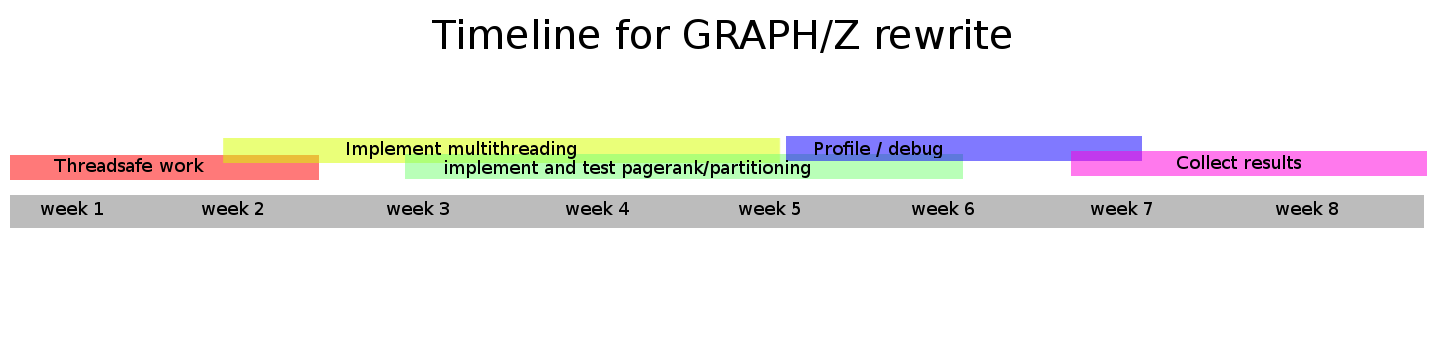
\includegraphics[width=\textwidth]{timeline.png}
\begin{multicols}{2}
  \section{Deliverables}
   The main component of the deliverables will be a poster outlining the new GRAPH/Z's strengths and weaknesses and highlighting the changes that we made from the original project. The poster will also include the abstract and writeup needed for entering it into the Supercomputing conference.  Deliverables will also include the finished GRAPH/Z processing system and information comparing it to GraphLab and other existing similar tools. Also included with be data from profiling and traces. 
   \section{Conclusion}
   The original GRAPH/Z was underperforming compared to most other productions graph processing systems. We hope by rewriting it from scratch with a new backend storage system we will discover what may be the cause of the lack of performance. In order to determine if the ZHT distributed hash table is an IO bottleneck, we will confine our implementation to a single node, and use an alternate backend besides ZHT.


   \bibliographystyle{plain}
   \bibliography{cite}
\end{multicols}
\end{document}
